Awesome

We can generate a new world, with different terrain and placement of bushes, trees, forests and volcano. A world with 0.5 vertex density takes about 23 ms on a single 3.4 GHz Intel i5 core, which is fairly fast. The world looks very nice both close, however with tesselation even more so, and both far and very far away. An example of a world seen from far above is shown in figure \ref{fig:worldFromFarAbove}. The forests and the nature look really good compared to many games. It is a very fine foundation to build a game on, either a FPS or even a RTS or RPG, since it looks good at all ranges and the world can be big enough. With further work such as LOD levels for the vegetation and tesselation for the land, even vaster and richer worlds could easily be made.
\begin{figure}[H]
  \centering
  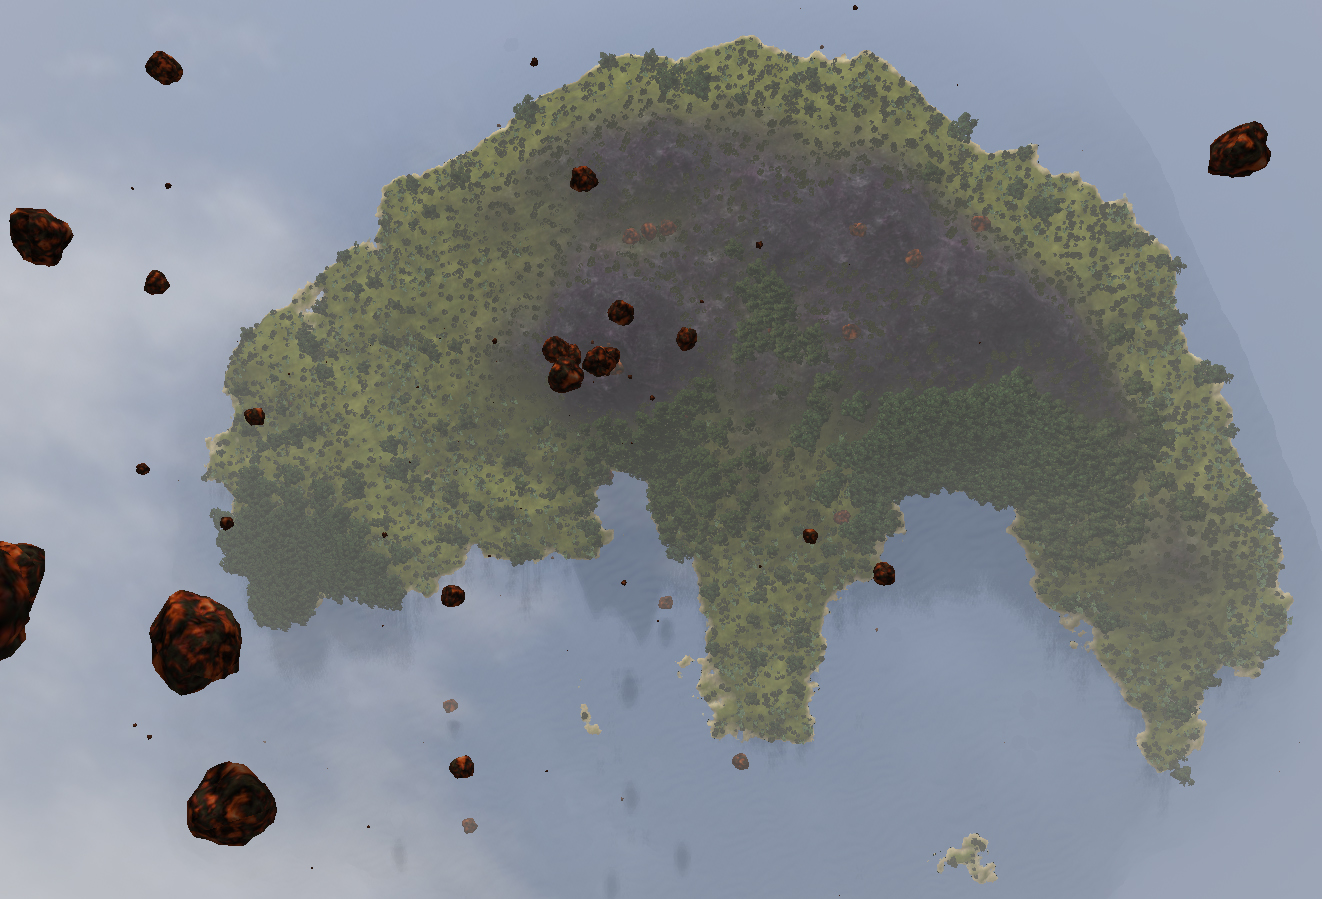
\includegraphics[width=\linewidth]{images/worldFromAFarTop.jpg}
  \caption{The final world from far above.}
  \label{fig:worldFromFarAbove}
\end{figure}%

Possible improvements:\\
* LOD (for the vegetation)\\
* Tesselation (terrain)\\
* Living water with real waves (using tesselation)\\
* Segmentation of the world, e.g. using an occtree, to speed up the collision detection.\\
* Inhabitants of the world?
















